%!TEX root = ../thesis.tex
\chapter{Results and Discussion} % (fold)
\label{cha:results}
In this chapter we will go through our experimental setup and results followed by a detailed analysis and comparison with relevant work.

\section{Experimental Setup} % (fold)
\label{sec:Implementation}

For implementation of our methodology, we used a Dell T7910, Dual Xeon Processors E5-2680 V4 @ 2.4GHz, RTX 3080Ti GPU, 32GB RAM, Ubuntu 20.04 Operating System as shown in Figure \ref{fig:experimental-setup}. We installed the CUDA matrix library to access GPU-based matrix operations to be able to run required parts of GPU computation. We installed a GPU-accelerated primitives library for DNN called NVIDIA CuDNN which provides highly fine-tuned standard routines implementations like forward-backward convolution, pooling, normalization, and activation layers which gives effective performance with CNNs.

We used Kaldi ASR \cite{daniel_povey_kaldi_nodate} Toolkit for the preparation of Language and Acoustic Models and Training of ASR (using Chain nnet3 CNN-TDNN) as shown in Figure \ref{fig:implementation-architecture}. Kaldi is an open source research speech recognition toolkit that implements many state-of-the-art algorithms. Kaldi is currently one of the most tested and cited ASR engines with a very supportive open-source community dedicated to the development and expansion of the project. Various sources show that it still outperforms its contemporaries \cite{christian_gaida_comparing_2014} \cite{georgescu_performance_2021}.

Dataset was divided into test and train as explained in section \ref{sec:Data_preprocessing}. Language Models were prepared using SRILM as explained in section \ref{sub:language_model}. Audio slicing and pre-processing were done using SoX, FFMPEG and Audacity. Monophone and Triphone HMM-GMM Training utilized Open FST, ATLAS and BLAS/LAPAC libraries where as in the Chain CNN-TDNN we used NVIDIA's CUDA and CuDNN for GPU Computation. The scripts used in this were mostly bash, C++ and Python. 

%It has scripts in various languages like C++, bash, perl, python etc. We needed a system that could use the relevant model files from Kaldi and make it easy to deploy in a client-server environment. Kaldi is in C++ primarily and since most of the applications now are python based, we wanted a python based solution for better ease of cross-platform deployability.

ASR Model training produces a lot of Language and Acoustic Model Files which can be an issue during deployment and leads to cross-platform compatibility problems which is why we needed a STT interface that could utilize the model files and give us flexibility and ease of deployment for which we used an open-source offline STT tool called Vosk \cite{alphacep_vosk_2022}. This required us to have python available since this portion is primarily python based.

\newpage
\begin{landscape}

\begin{figure}[htbp]
    \centering
    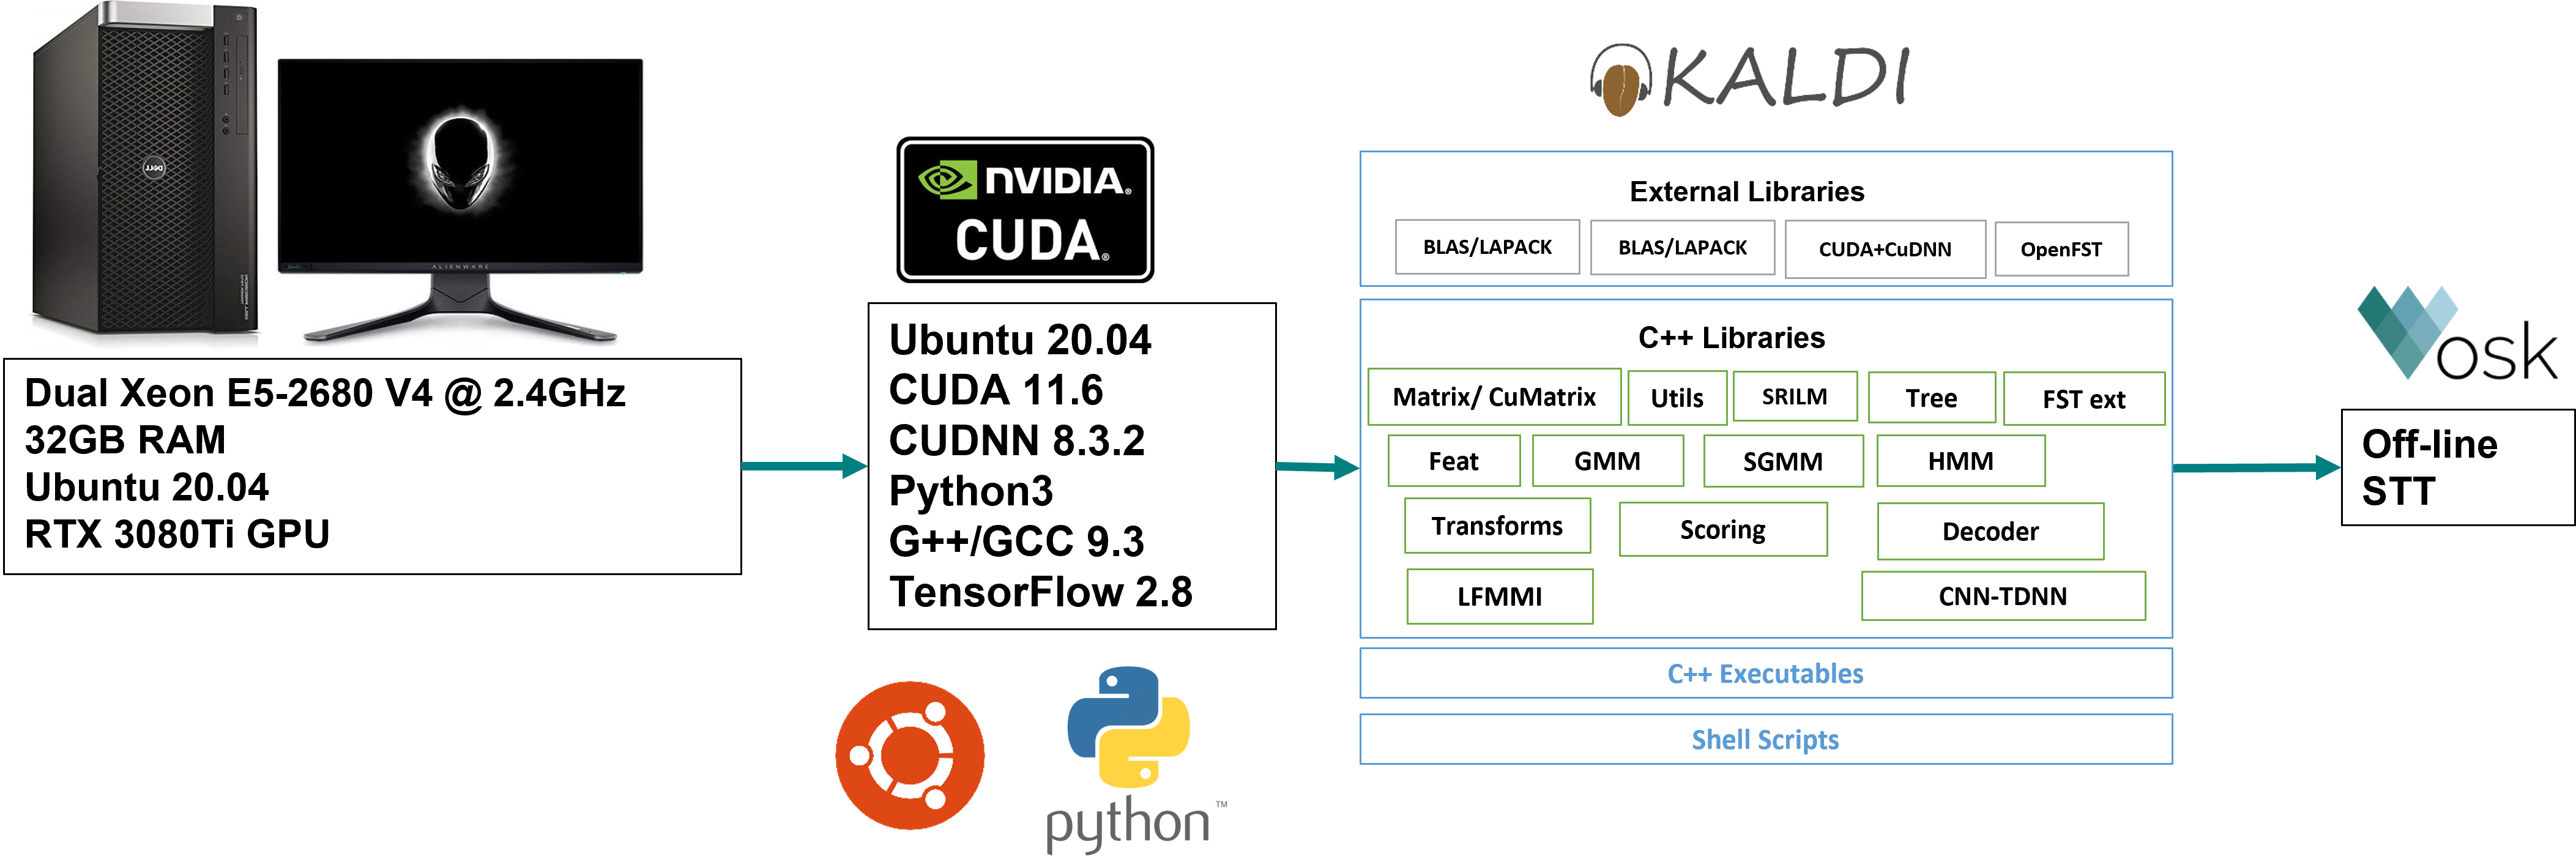
\includegraphics[width=1.5\textwidth]{img/Implementation.png}
    \caption{Experimental Setup}
    \label{fig:experimental-setup}
\end{figure}
\newpage
\begin{figure}[htbp]
    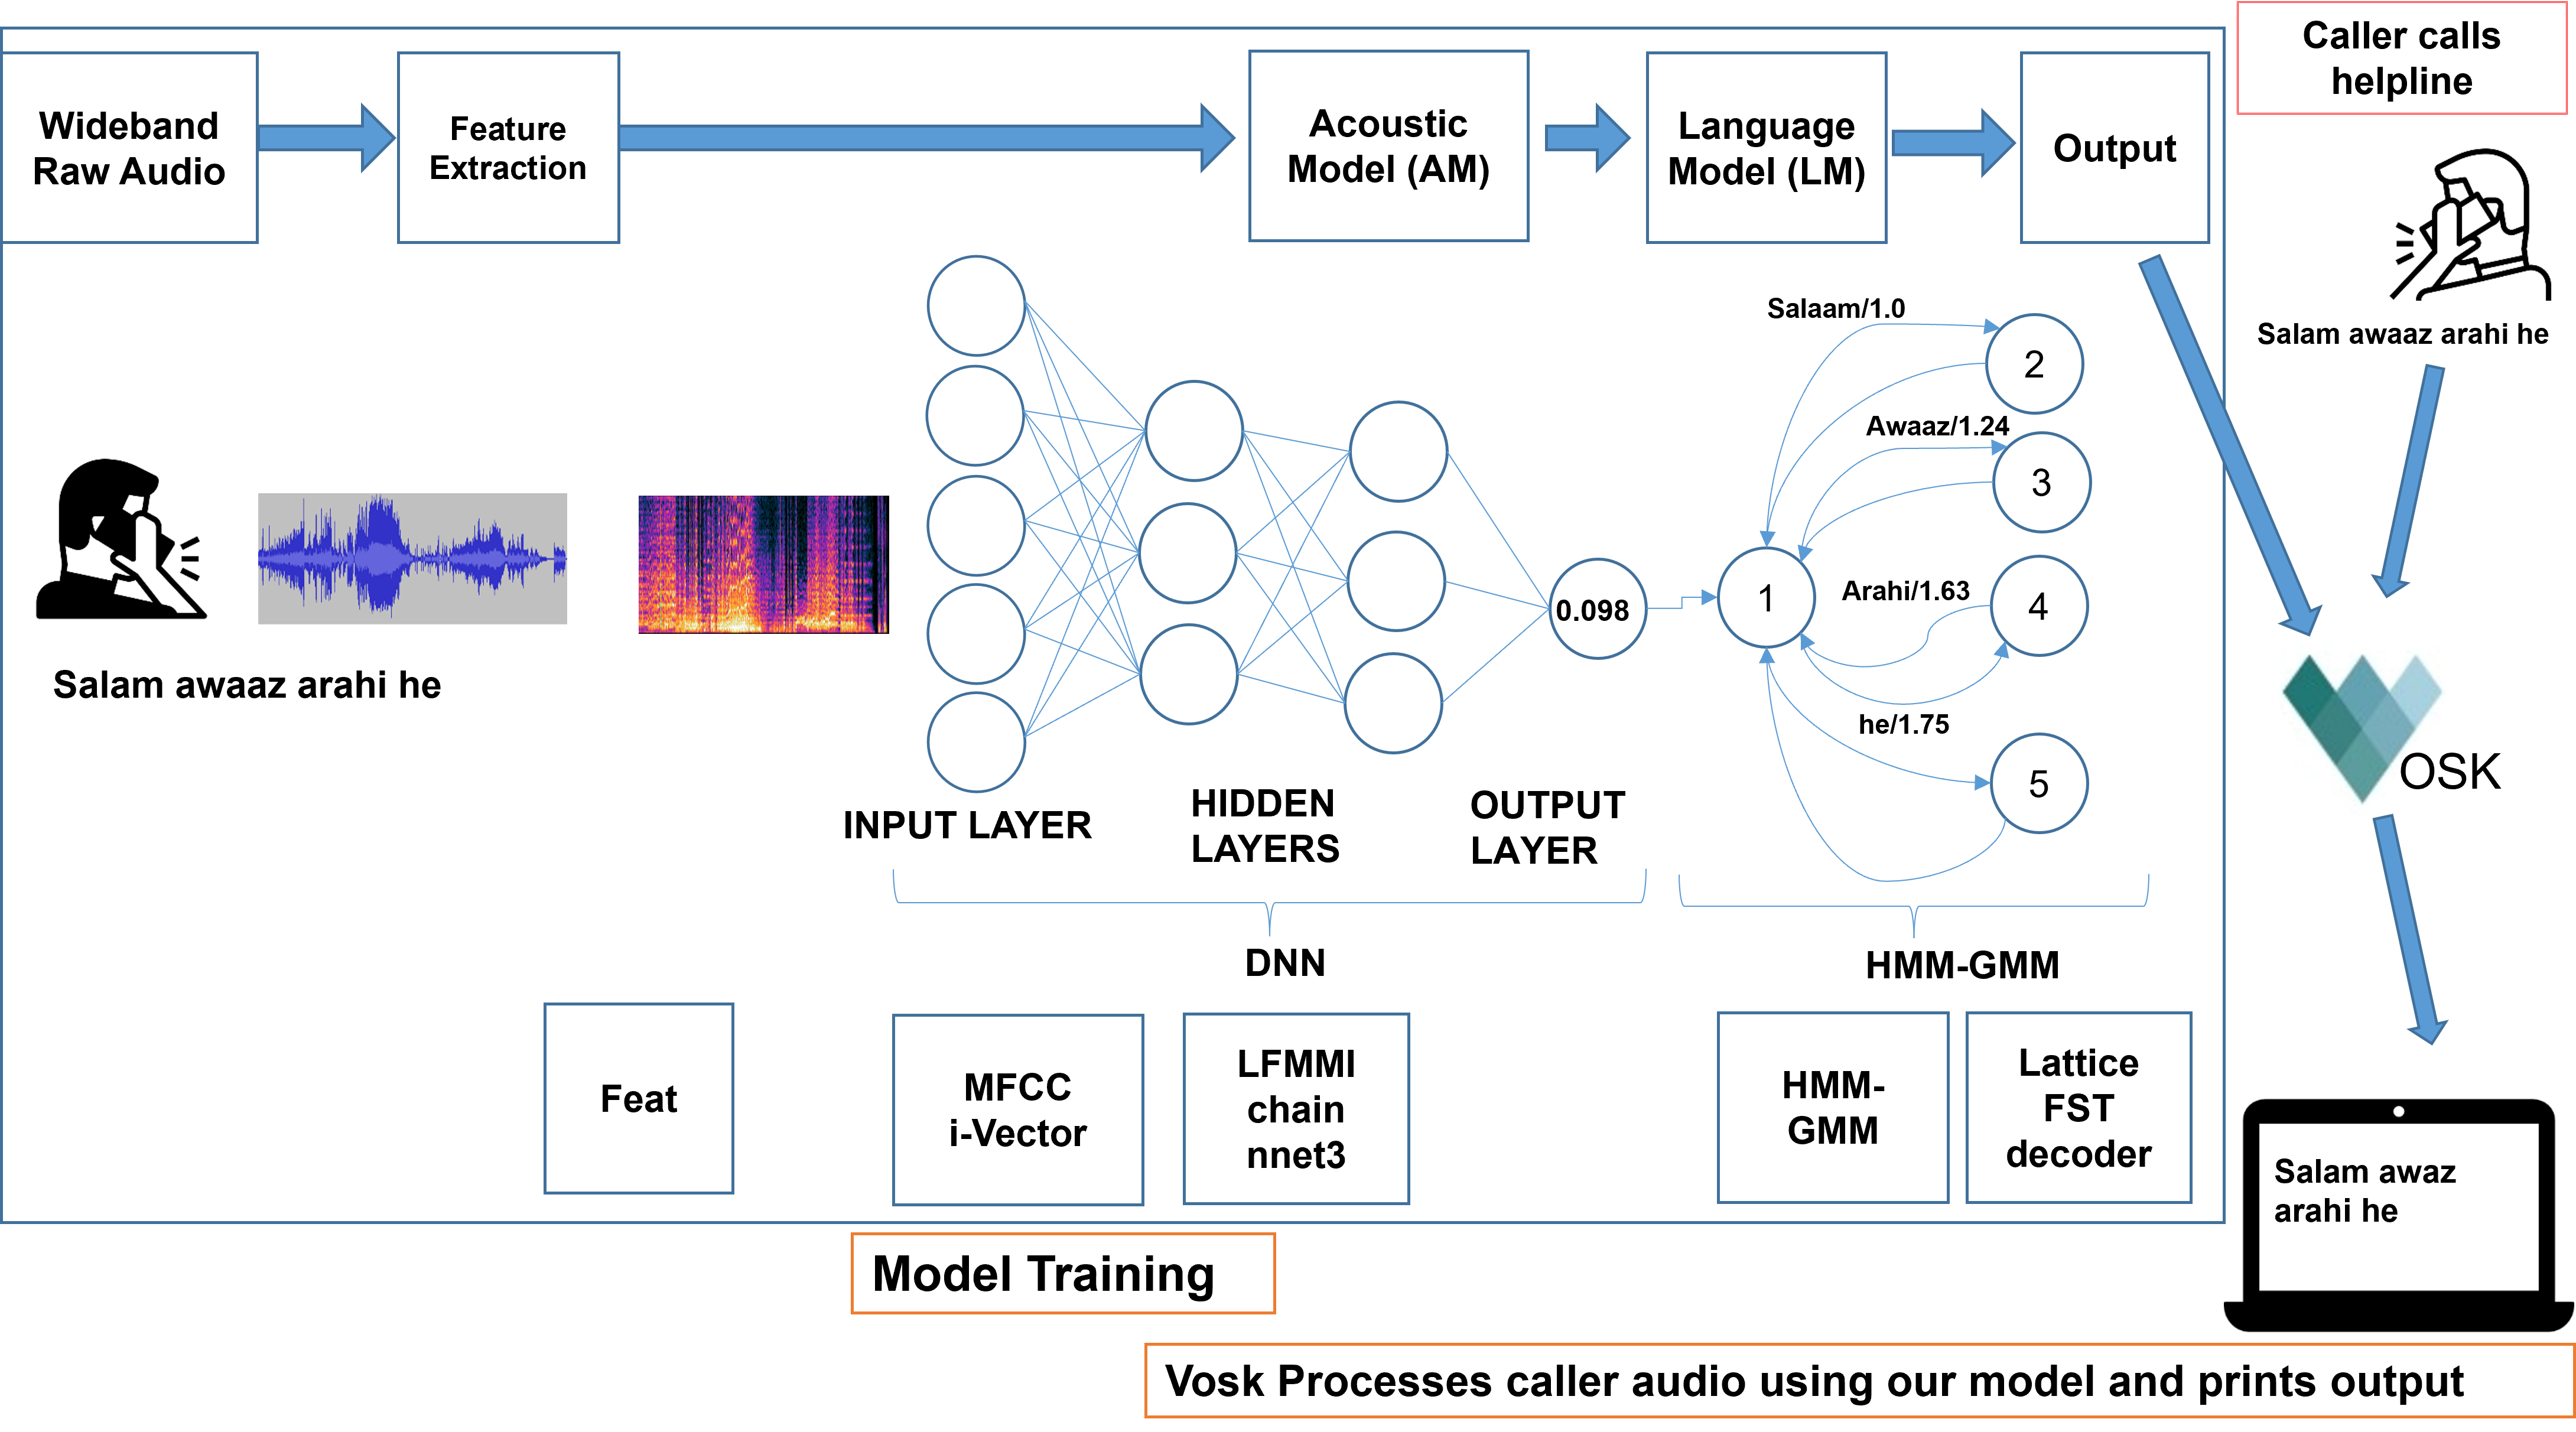
\includegraphics[width=1.5\textwidth]{img/Implement2.png}
    \caption{Implementation Architecture}
    \label{fig:implementation-architecture}
\end{figure}

\newpage
\end{landscape}

\section{Experimental Results}

\begin{table}[h!]
    \centering
    \caption{Our Results} 
    \label{tab:our_result}

    \begin{tabularx}{\textwidth} { 
  | >{\raggedright\arraybackslash}X 
  | >{\raggedright\arraybackslash}X 
  | >{\raggedright\arraybackslash}X | }
    \hline
    \textbf{Data-set} & \textbf{METHOD} & \textbf{RESULTS} \\
    \hline
    Data-set \ref{sub:datasources} D(1-4) & HMM GMM TRIPHONE & WER 13\% and SER 31.2\%  \\ 
    \hline
    Data-set \ref{sub:datasources} D(1-4) & LFMMI CNN-TDNN & WER 5.2\% and SER 20.45\%  \\
    \hline
    Data-set \ref{sub:datasources} D(5) & LFMMI CNN-TDNN & 5.2\%\\   
    \hline
    \end{tabularx}    
\end{table}

We were able to acheive 13\% WER and SER of 31.2\% using HMM-GMM and with CNN-TDNN using LFMMI Objective Function we achieved 5.2\% WER and 20.45\% SER on clean and noisy code-switched Urdu audio data with read speech, spontaneous speech, isolated words and isolated digits. The details of our results is shown in table \ref{tab:our_result}. 

For Evaluation we used WER and SER. While the option of using CER was there we found it irrelevant for us since we are more concerned with the accuracy of words and sentences. The Urdu word \textit{"Janbaaz"} can also be written as \textit{"Jaanbaaz"} or \textit{"Jaanbaz"} and will be spelled pretty much in the same way. Hence, as long as the overall word is accurate and the sentences are accurately transcribed, our ASR is suits our requirements.

It must be noted that Call center audio used for testing was totally unseen, containing OOVs, overlapping and low-volume speech. In audible speech signal areas with no overlap and clean speech (whether single word or long sentences) we were able to achieve WER 5.2\%. but in the overlapping areas, lower volumes, incomplete or partial speech by the speaker and OOVs, the performance degraded yielding 74\% result. 

\section{Comparison with Relevant Work} % (fold)
\label{sec:comparison_result}

For comparison purpose, we used only WER as evaluation metric since we only had WER available in those work as shown in Table \ref{tab:comparison-table}. Our Call Center data is not openly available and hence cannot be used as a metric to compare performance with others. However we can use \cite{ali_automatic_2015}, \cite{sehar_gul_detecting_2020} and \cite{qureshi_urdu_2021} for bench-marking since their data was available and applied in works other than ours. 

%The catch is that most of these tests were conducted using the same set of audio recordings: namely a corpus called Switchboard, which consists of a large number of recorded phone conversations spanning a broad array of topics. Switchboard has been used in the field for many years and is nearly ubiquitous in the current literature—so it’s a reasonable choice. By testing against the same audio corpus, researchers can make apples-to-apples comparisons between themselves and competitors. (Google is the exception; it uses its own, internal test corpus, which is opaque to outsiders).

All these works focused on one of the aspects of ASR input i.e. read speech, isolated words or digits and spontaneous speech. In our case all of these scenarios were covered which makes it more applicable in practical sense.

The works in comparison were all tested primarily on clean audio, making it unsuitable for noisy telephonic environment. In our case the model performed with 5.2\% WER in noisy and clean environment. However in overlapped, improper pronunciations and low volume speech, our model was unable to perform well.

These works focused on pure Urdu words which means they are not applicable for telephonic environment since languages are spoken in code-switched manner. We were able to identify words usage patterns based on Call Center scenario to cover maximum possible vocabulary, trained with noisy and clean samples of same word set to cover maximum possible scenario. We also solved the code-switching problem by keeping a unified written script i.e. Roman. So all English or Urdu words were in Roman script which eased the lexicon building and language modelling process. 

One of the drawbacks of \cite{sehar_gul_detecting_2020} that we identified was that it used very little data-set to train Urdu ASR with Deep Learning. In our case we had limited access to labelled dataset and most of our dataset was unlabelled for which we trained a Hybrid HMM-DNN ASR which was able to use statistical alignments and Neural Networks to train accurate ASR on limited dataset. This approach is suitable for Low-Resource Languages where labelled dataset is not easily available.

Other works mentioned in Chapter \ref{cha:literature_review} cannot be fairly compared (though provided as a reference for bench-marking in future based on available data) because the data-sets are not consistent. For that kind of comparison we need a data-set for Urdu like \cite{godfrey_switchboard_1992}, \cite{garofolo_john_s_timit_1993} and \cite{panayotov_librispeech_2015} on which we can apply various models with same experimental environment and conditions. The results from those training on the common dataset will be able to prove which model works best in noisy/ telephonic environment for Urdu Language. A performance comparison like \cite{georgescu_performance_2021} can then be done on the common data-set for better comparison and analysis.

\begin{landscape}
 
\begin{xltabular}{1.5\textwidth}{|l|X|X|X|}
\caption{Comparison with relevant work} \label{tab:comparison-table} \\

\hline \multicolumn{1}{|c|}{\textbf{Author}} & \multicolumn{1}{c|}{\textbf{Data-set}} & \multicolumn{1}{c|}{\textbf{Method}} & \multicolumn{1}{c|}{\textbf{Reults}} \\ \hline 
\endfirsthead

\multicolumn{4}{c}%
{\tablename\ \thetable{} -- continued from previous page} \\
\hline \multicolumn{1}{|c|}{\textbf{Author}} & \multicolumn{1}{c|}{\textbf{Data-set}} & \multicolumn{1}{c|}{\textbf{Method}} & \multicolumn{1}{c|}{\textbf{Results}} \\ \hline 
\endhead

\hline \multicolumn{4}{|r|}{{Continued on next page}} \\ \hline
\endfoot

\hline
\endlastfoot
    Our Work & Data-set \ref{sub:datasources} D(1-5) & HMM GMM TRIPHONE & WER 13\% and SER 31.2\%  \\ 
    \hline
    Our Work & Data-set \ref{sub:datasources} D(1-5) & LFMMI CNN-TDNN & WER 5.2\% and SER 20.45\%  \\   
    \hline
    Qasim \cite{qasim_urdu_2016} & 139 District names of Pakistan, 300 speakers & HMM & Accent Dependent 60.06\% \newline Accent Independent 75.25\% \\
    \hline
    Hazrat Ali \cite{ali_automatic_2015} & 205 isolated words (20 Speakers) & HMM &  WER 33\% \\
    \hline
    Sehar Gul \cite{sehar_gul_detecting_2020} &  250 words each by 10 speakers \newline 86 sentences by 25 people \newline 100+86 sentences 25 people \newline & Deep Learning (E2E CTC) using DeepSpeech & Accuracy 60\% \newline 56.7\% \newline 51.6\% \\
    \hline
    Zoraiz Qureshi \cite{qureshi_urdu_2021} & PRUS\cite{zia_pronouncur_2018} 708 sentences data set with 5 speakers & GMM/HMM& Accuracy 65\%-75\% (WER 25-35\%) \\
    \hline
    Naeem \cite{naeem_subspace_2020} & Dataset by RUMI and CSALT and NUCES - clean Mono-16000Hz & MONO \newline Tri-1 \newline Tri-2 \newline Tri-3 \newline SGMM \newline (HMM-GMM-SGMM) & WER 3.24\% SER 64.26\% \newline WER 16.70\% SER 52.41\% \newline WER 16.74\% SER 52.80\% \newline WER 13.63\% SER 52.62\% \newline WER 9.64\% SER 48.53\% \\
    \hline
\end{xltabular}
\end{landscape}

\section{Analysis of Results}
\label{se:discussion}

From the perspective that we set out initially to improve work of \cite{sehar_gul_detecting_2020}, our model has clearly out-performed on Sehar's Data-set of malicious Urdu sentences and on general code-switched Urdu conversations as well. 

The works we studied for Urdu ASR were tested to perform generally in clean environment on one of the following: Isolated words, Isolated Digits, Read speech or spontaneous speech. Our work was able to perform with 95\% accuracy on all these types of speech in a noisy as well as in clean environment. We found that most of the previous work generally focused on using pure Urdu words or sentences. The fact remains that Urdu is never spoken in pure form. It is always spoken in code-switch to English, Panjabi and other local languages as well in normal conversation. 

\subsection{Addressing Code Switching issue}

The usual idea for speech to text output may be to use local script for the transcription text and in Urdu it is usually Nastaliq. However, to address the code-switching issue we kept the written script as Roman instead of making Urdu Nastaliq and Roman English separately allowing us to bypass the requirement of building separate Language and Phonetic Models for every word of a different language used. Keeping one writing script for code-switched Low resource language will help solve the issue of Language modelling, saving a lot of time to structure and map data, while also reducing the Model complexity. 

Our Model was able to recognize numbers and write them down in Arabic Numeral scripts which was due to the fact that we mapped the numbers to their pronunciations in our Lexicon. In situations where the speech include series of number, the ASR used arabic numeral as text output instead of their English pronunciation which is a result we have not seen before in a code-switched Urdu ASR. 

\subsection{Data Centric Approach}

Based on our results, our approach clearly out-performed the usual model-centric approach. We built our ASR from scratch which meant that Data Pre-Processing also has to be iteratively audited (as seen in figure \ref{fig:datacentric-ML-approach}) along with model tweaking. This is one of the key reasons why our model performed better.It also provided us following advantages \cite{noauthor_data-centric_nodate}:
\begin{itemize}
    \item Improved accuracy by effectively using data as a strategic asset to ensure more precise estimates, observations, and decisions.
    \item Complex data transformations are eliminated.
    \item Data inconsistencies and errors are reduced.
    \item Data redundancy is reduced.
    \item Data quality and reliability is improved.
    \item Expenses are reduced since less time and effort is required to work on model building and tweaking.
\end{itemize}

\subsection{Data-set Diversity}

We added a unique diversity in our data-set which covered maximum possible scenarios in our call center ASR. Our data performed optimally in all the following points (English and Urdu):
\begin{itemize}
    \item Isolated Digits
    \item Isolated words 
    \item Urdu Malicious sentences (Section \ref{sub:datasources} from D2)
    \item Read Speech (Words and Digits) of duration up to 20 seconds
    \item Spontaneous Speech (Words and Digits) of duration up to 20 seconds
    \item Clean Audio
    \item Noisy or Telephonic Audio
    \item Audio lengths. The feature extraction of the input signal is limited by the memory of GPUs in use, it is best to slice all audio files not to exceed 30 seconds, as it is a reasonable input size for batching.
\end{itemize}

Other models we studied in our literature review performed in on or two of the above points. Our model is the first that covers all these scenarios. This model works as a speaker independent model.

The best approach for a resource constraint scenario is to take small data-set of 10-20 hours. We accurately label it to build a strong language model. It is best to understand the context of data-set and do an analysis of the language usage e.g. for code-switching, common words, jargon etc. Then train a strong model which can then annotate the remaining data-set which can then be used to train Deep Learning Model which is known to improve as data-set size increases. The golden data-set we will eventually have as we accurately label and integrate more and more data will become our asset. 

Models will evolve for the better but data-set is the same (mostly a standard). Hence it is always best to build up the data-set instead focusing on model only.

\subsection{The Role of Chain CNN-TDNN Approach}
HMM-DNN method involves use of statistical model to build up Language and acoustic models. These alignments can be used to further train and improve model using Neural Networks. In a way it uses the accuracy of Statistical Models on low data-sets and the scalability of Neural Networks together. 

We used CNN-TDNN for Neural Network Training with LF-MMI Objective function which has previously shown to work better on noisy data-sets \cite{daniel_povey_kaldi_nodate}\cite{abdel-hamid_convolutional_2014} \cite{zorila_investigation_2019} \cite{biswas_semi-supervised_2019} \cite{noauthor_tdnn_nodate} \cite{georgescu_kaldi-based_2019} \cite{kreyssig_improved_2018}. This architecture has CNN Layers followed by TDNN Layers which both add certain benefits in the Training pipeline.

If the input features are noisy, having a few CNN layers (2D CNN) before TDNN (which is basically a time dialated 1-dimension CNN) blocks at the input would help the model learn some non-linear transformations which can reduce the effect of the noise on speech input. TDNNs are basically temporal convolution whereas CNNs are convolutions in both frequency and space dimensions, which gives it the capability to learn patterns better.

TDNN works well in Speech Processing compared to other Neural Networks as they can be tuned easily as compared to LSTMs, and gives 11.4\% WER than the baseline TDNN's 12.1\% WER on the Switchboard \cite{godfrey_switchboard_1992} part of Eval2000 data-set \cite{daniel_povey_kaldi_nodate}. 

Speech Recognition requires a system that takes care of temporal context and time delay neural network architecture captures long term temporal dependencies better than a feed-forward DNN does. We need to look at features left and right i.e. contexting and we need better prediction of phoneme states which is why for Low Resource Languages TDNNs work best. 

The LF-MMI or chain model helped reduce the training time of the model and allowed for more efficient and effective training which improved accuracy from HMM-GMM Triphone training by 8\% in our case. It makes best use of GPU and avoids using branching or pruning tree search. 

The process of creating the denominator FST is very similar to that of a traditional decoding graph creation, however the computation of the denominator forward-backward computation are parallelized by the GPU. The process is sped up by performing careful optimizations, including reversal, weight pushing, and minimization followed by epsilon removal on the denominator FST to minimize graph size.

Hence this reduces graph size and improves training speed an performance while using Neural Networks, in comparison to pure Deep Learning based models. It is also applicable on streaming data.

%This model can be trained directly without word lattice of pre-training because LF-MMI uses:
%\begin{itemize}
%\item Phone Level Language Model usually 4-gram instead of 
%\item No LM Smoothing to avoid introduction of multiple states
%\item 30ms frames in feature extraction instead of 10ms
%\item One state per phone instead of 3   
%\end{itemize}

\subsection{Speech To Text System Interface Integration}
We identified based on relevant work from our literature review that Model Files that are generated are often huge in Size which causes difficulty in deployment. Our proposed framework utilized a Speech To Text Interface that would use relevant files giving it flexibility, ease of cross-platform deployment and scalability \cite{alphacep_vosk_2022}.

Using Kaldi and Vosk \cite{alphacep_alphacepvosk-server_2022} allows us to built accurate offline speech recognition supporting four major communications protocols i.e. MQTT, GRPC, WebRTC, and Websocket. Server can be locally used to provide speech recognition to smart homes and PBXs such as free-switch or asterisk and can also deployed as a back-end for web-based streaming speech recognition, as well as to power chat-bots, websites, and telephony.

%The idea behind STT interface like Vosk is that the neural network-based speech recognizers require a huge amount of speech data for training and enormous computing power and time to train and optimize the parameters. Neural networks have problems with human-like one-shot learning, their decisions are not very robust to unseen conditions and are hard to understand and correct. 

%Thus, a system based on large signal database concept was built in which audio fingerprinting scheme is applied. The audio is segmented on chunks, the chunks are stored in the database based on LSH hash value. During decoding the system looks up the chunks in the database to get the possible phones which helps it to make a proper decision on decoding results.

%Neural network-based speech recognizers require a huge amount of speech data for training and enormous computing power and time to train and optimize the parameters. Neural networks have problems with human-like one-shot learning, their decisions are not very robust to unseen conditions and are hard to understand and correct. 

%Thus we need a system that is built based on large signal database concept in which audio fingerprinting scheme is applied. The audio is segmented on chunks, the chunks are stored in the database based on LSH hash value. During decoding the system looks up the chunks in the database to get the possible phones which helps it to make a proper decision on decoding results.

%The \textbf{advantages} of this approach are:
%\begin{itemize}
%    \item It can quickly train on more than ten thousand hours of speech data on very simple hardware
%    \item It can easily correct recognizer behavior just by adding samples
%    \item It can make sure that recognition result is correct because it is sufficiently represented in the training data-set
%    \item It can parallelize training across thousands of nodes
%    \item It supports lifelong learning paradigm
%    \item It can use this method together with more common neural network %training to improve recognition accuracy
%    \item The system is robust against noise
%\end{itemize}

\section{Shortcomings}
\label{sec:shortcomings}
The Shortcomings can be categorized into following:
\begin{enumerate}
    \item Robustness 
    \item Data-set Limitations
    \item Model Limitations
    \item Speech To Text Interface Limitations
\end{enumerate}

\subsection{Robustness}
Our ASR system faced issues with accuracy in overlapping speech and in longer duration audios. The problem of overlapping speech  is still one of the most difficult in ASR \cite{chen_progressive_2018} and it must be catered in this system. Eventually it will be desirable to go towards E2E solutions which do not require the language structuring. 
\par
However, that can only be done once we have more than 1000 hours of data of labelled speech which is in itself a big project. Without consistent data-set, there is not much that can be said with authority as to which Language or acoustic modelling method works best for Urdu. 
\par 


\subsection{Data set Limitations}
We lacked a standard big data of labelled corpus like Switch Board \cite{godfrey_switchboard_1992} due to which it is not possible to benchmark or compare our performance to other works. Making a standard labelled big data in code-switched Urdu will be very beneficial for researchers working in Urdu ASR. It will help benchmark the performances of various models since data is standard. Roman and Arabic-based Urdu script are required with the audio model to help propel this area of research forward.

\subsection{Limitations of Model}

While HMM-DNN continues to produce cutting-edge results, DNN's role is limited. HMM-DNN has its own limitations which include:
\begin{itemize}
    \item DNN has a limited role and is mostly used for simulation of the posterior state probability of an HMM's hidden state. The time-domain feature is still being modelled by HMM.
    \item Data alignment problem arises when attempting to model time-domain features with RNN or CNN instead of HMM since loss functions of RNNs and CNNs are defined at each point in the sequence, hence the alignment relationship between the RNN output sequence and the target sequence must be known in order to perform training \cite{backstrom_introduction_2022}.
    \item It has a complex structure that includes several components such as the acoustic model, language model, and pronunciation model. Each system component is independently optimized with a different objective function, usually resulting in a suboptimal global solution. Hence, it requires linguistic resources like a handcrafted pronunciation dictionary prone to human error \cite{hussein_arabic_2022}. 
    
\end{itemize}

\begin{figure}[htb]
    \centering
    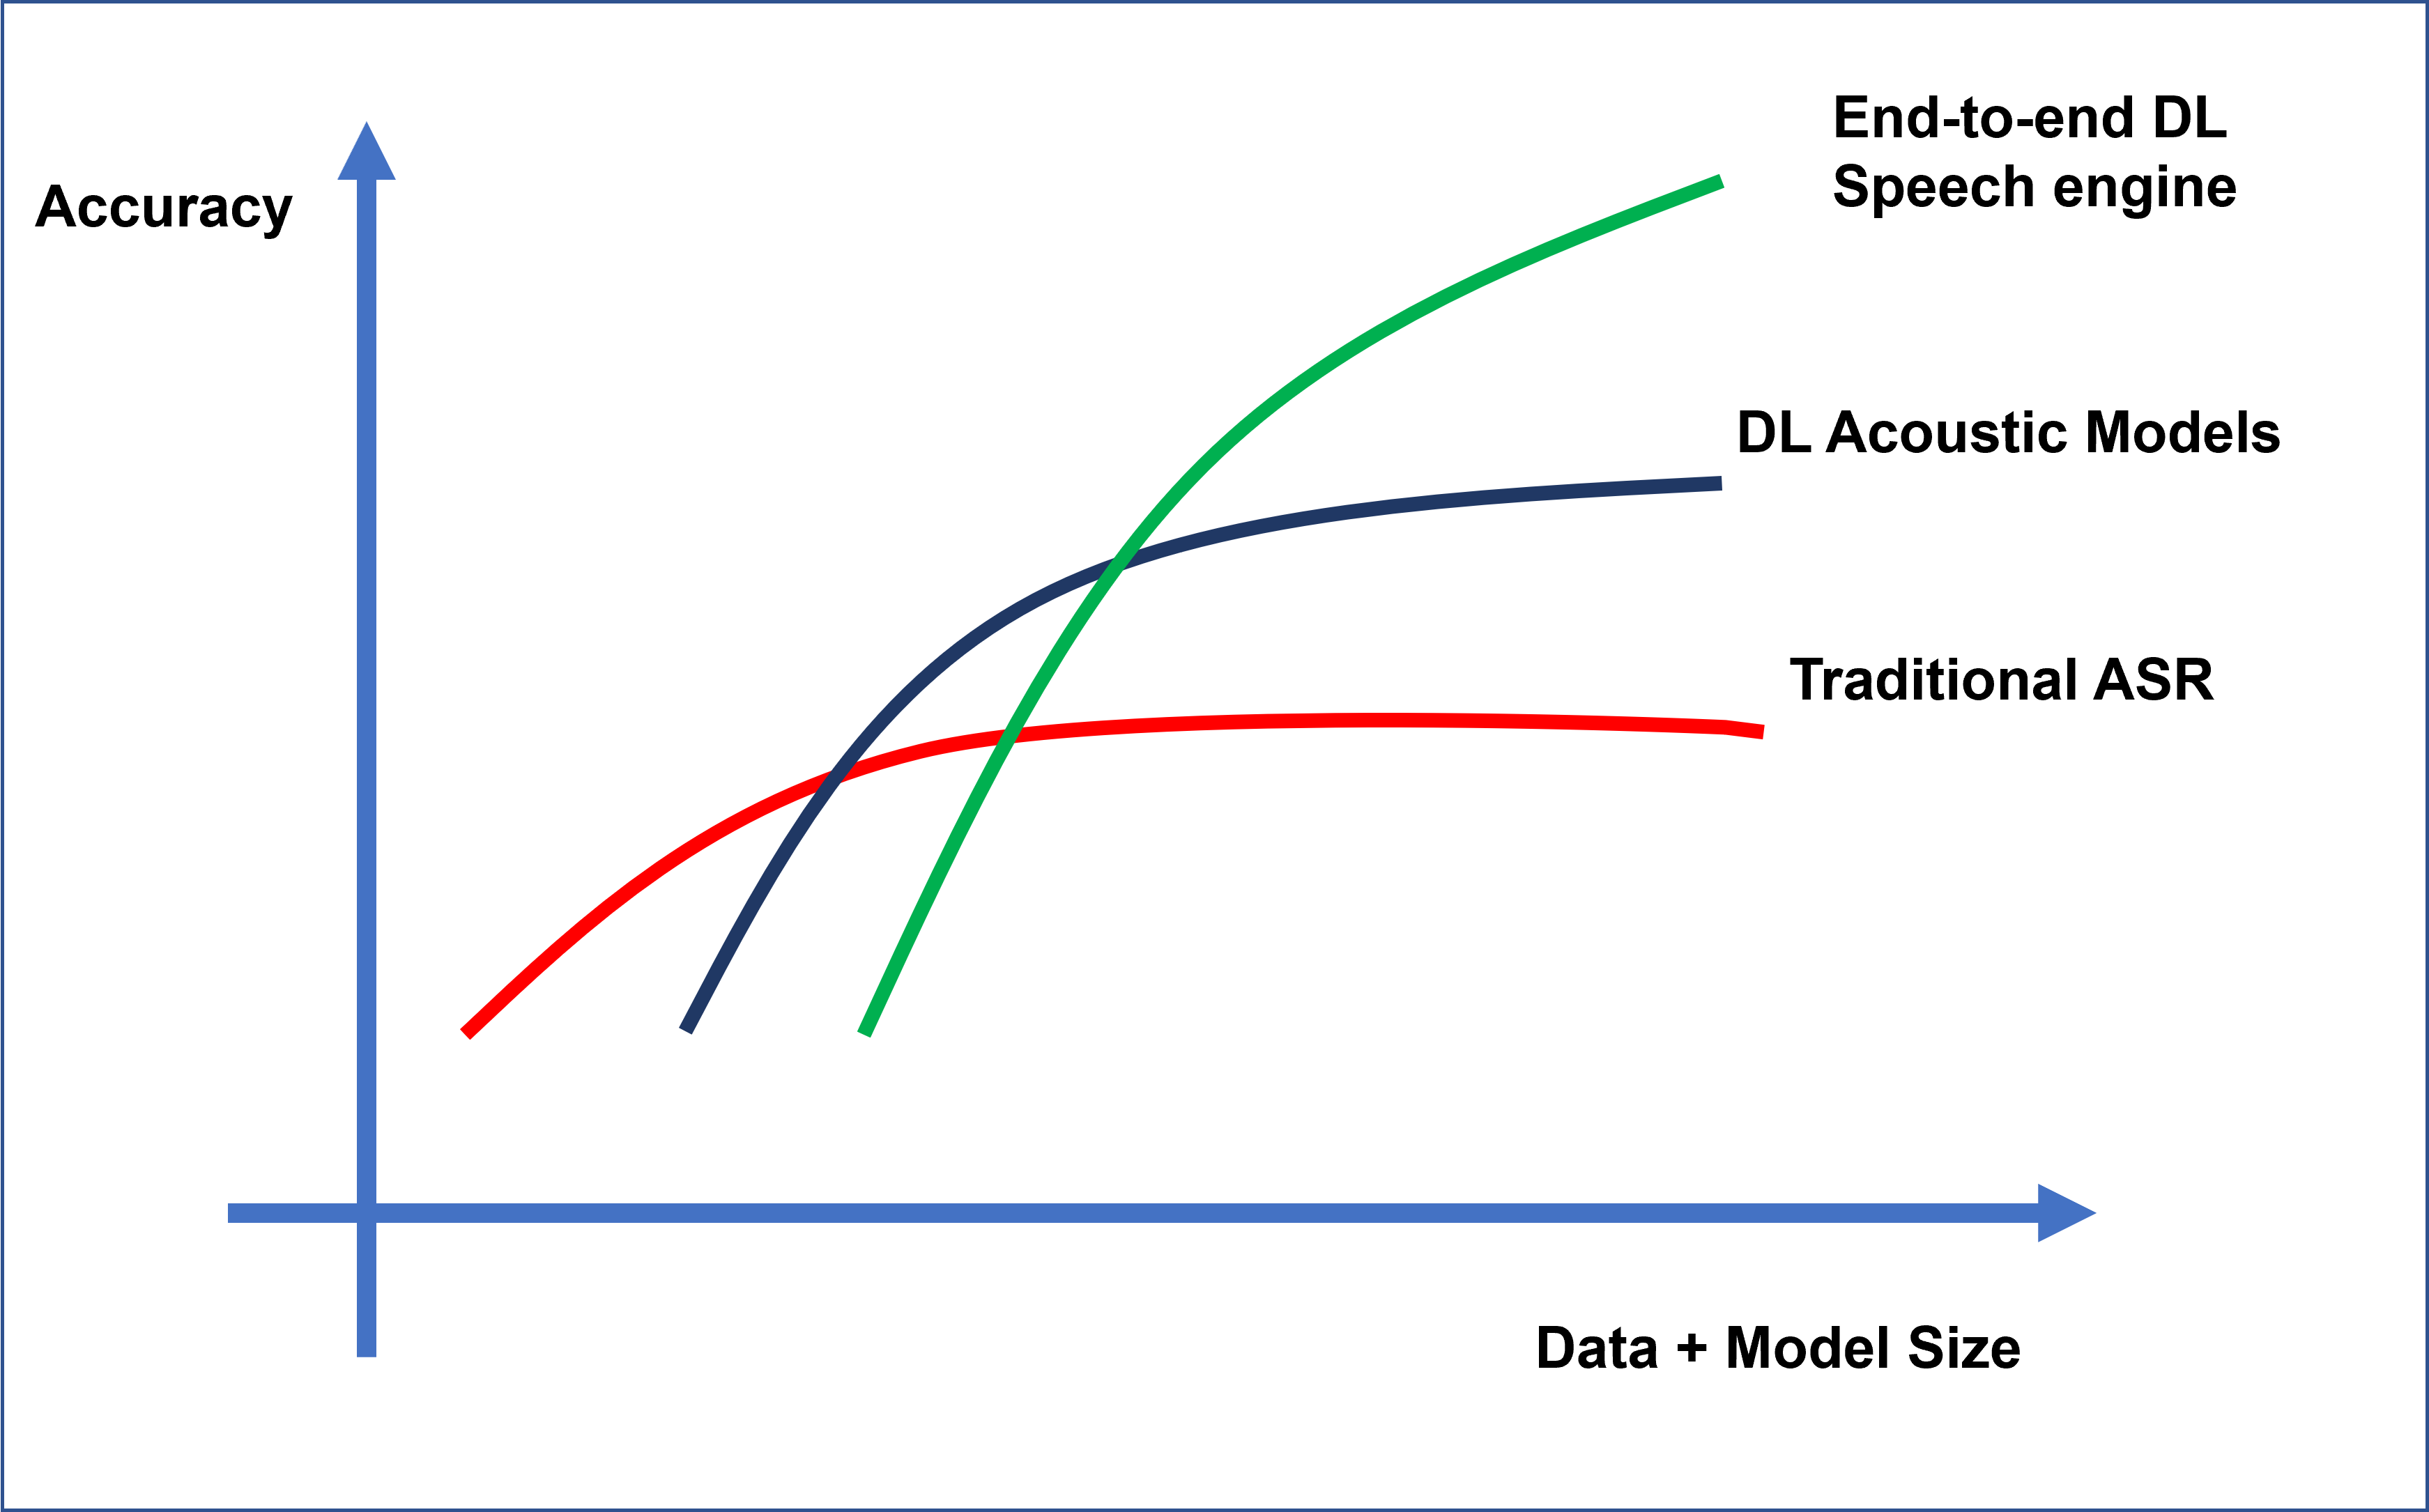
\includegraphics[width=0.8\textwidth]{img/ComparisonASRMODELS.png}
    \caption{Comparison of Three ASR Training Approaches} %For lower training datasets Traditional methods work well but E2E outperforms with bigger training data-sets.}
    \label{fig:comparison-all-asr-approach}
\end{figure}

\subsection{Speech To Text Interface Limitations}
We designed the system for use in a desktop or high-end client-server environment but the best usage of this will be deployment in edge devices as the world moves towards Edge computing and Internet of Things. This model at present is not deployed for self-supervised learning and federated machine learning or life-long learning method \cite{dautume_episodic_2019} \cite{chang_towards_2021}.

%It is built based on large signal database concept in which audio fingerprinting scheme and the \textbf{disadvantages} to this approach are \cite{alphacep_vosk_2022}:
%\begin{itemize}
%    \item The index is really huge, it is not expected to fit a memory of single server.
%    \item The generalization capabilities of the model are quite questionable, at the same time the generalization capabilities of the neural networks are also questionable.
%    \item For now the segmentation requires conventional ASR, but in the future we may need to segment it ourselves.
%\end{itemize}

\section{Future Work} % (fold)
\label{sec:future-work}

\begin{itemize}
    \item Model requires robustness in overlapping or distorted speech areas. To cater for robustness we will also need to expand this model to integrate approaches like Parametric and Adaptive models \cite{shrawankar_adverse_2013}. 
    \item Multilingual model training to integrate more languages which are locally spoken like Panjabi, Sindhi etc. The script can be kept Roman instead of Arabic to reduce language modelling complication.
    \item STT interface requires own code for segmentation of audio and it also requires Specialized hardware to implement this AI paradigm \cite{alphacep_vosk_2022}.
    \item Self-supervised training integration requires exploration  \cite{yang_online_2022}.
    \item Federated Learning and secure application on Edge AI systems need to be explored \cite{noauthor_federated_nodate}.
    \item Expansion of vocabulary, environment, accent and other variations in dataset is essentially required to form a golden dataset on which we can apply various training methods to get the most accurate model. 
    \begin{itemize}
        \item Data should be scaled up to more than 2000 hours eventually for better testing of End to End methods for Code-switched Urdu ASR. 
        \item Models change for the better but dataset is constant which is an asset. If we have a good dataset, we can always train better models with better accuracy and robustness. 
        \item Figure \ref{fig:comparison-all-asr-approach} shows that HMM based model works well with less dataset but with increase in data size, accuracy of Deep Learning is much more than HMM or hybrid models.
    \end{itemize}
    \item Examining Sub-word implementation \cite{smit_advances_2021} for code-switched Urdu and apply other Language Modelling methods like RNN, to test if this model can be improved.
        \begin{itemize}
            \item Slavic Languages e.g. Estonian, Nordic Languages E.g Finnish and Arabic Languages are highly inflected languages which requires specific components for modelling inflection e.g. factored language model. 
            \item An effective method is to use Sub Word Implementation \cite{smit_advances_2021} which has shown to improve accuracy more for Arabic language compared to English. 
            \item Arabic Language, as a case study, has a concept of base words comprising of three letters from which other words are derived.
            \begin{itemize}
                \item E.g. \RL{علم} (pronounced as Ilm) means knowledge which is base word. The word \RL{معلم} (pronounced as Mualim) means teacher or mentor, the connotation means transmitter or sharer of knowledge. 
                \item The essence and the characters or alphabets of the base word \RL{علم} (comprising of 3 alphabets "\RL{ع}" "\RL{ل}" "\RL{م}") remains there as the word compounds and expands. 
                \item If this structure is learned by the Computer through Machine Learning, Machines may be able to capture out-of-vocabulary words more easily. 
            \end{itemize}
        \end{itemize}
    %\item Building a Robust and noise resistant model is still one of the hard problems in ASR.
\end{itemize}


